\section{Behavior Design Patterns}

% Two columns start
\iftwocolumns
\begin{multicols}{2}
\fi

TODO:

\subsection{Chain of Responsibility}

(InputHandlers and InputDispatchers) in Frostbite engine. A series of input handlers are chained together. Each input handler may hold reference to other input handlers.
\bs
When an input, such as mouse, keyboard, or controller action occurs. The calls traverses down the chain of input handlers until one of the input handler entities "consumes" it, which ends the chain.
\bs

Another chain of command pattern observed in the Forstbite engine editor, is handling mouse press when there are multiple \textit{hitzones}\footnote{Hitzones are interactive areas for mouse that reports data and events such as mouse position, if mouse is hover, mouse button presses and releases} overlapped (figure \ref{fig:chainofcommand-mousezones}). Any press or hovering event will be handled by the top-most hitzone entity first. If the handler does not consume the input event, the event will naturally "flow" down to the next level.
\bs

\begin{figure}[H]
	\centering
	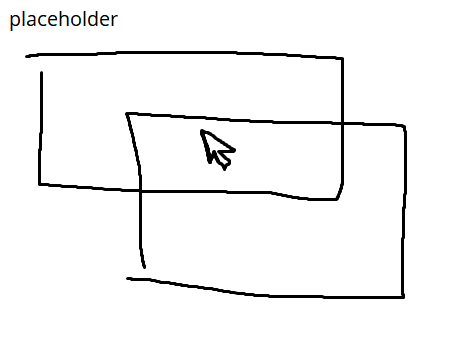
\includegraphics[width=0.3\textwidth]{assets/chainofcommand_mousezones}
	\caption{Mouse interacting with overlapping mouse hitzones}
	\label{fig:chainofcommand-mousezones}
\end{figure}

\subsection{Command}

Decouples action request and action handlers. The callee who makes the request makes no assumptions about the class the receives the command. Effectively decoupling them.
\bs
This opens up more flexibility in mapping a requests to a handler. An example is re-mappable input handling. Instead of listening for a key press, then calling a specific function that the key press corresponds to. It invokes a command object that holds a reference to the \textit{real object} so that the handler can be called.
\bs
In between we could do more things. For instance, keep track of how many times the action has requested.
\bs
Command pattern also opens up for redo/undo operations.

\subsection{Mediator}\label{ssection:mediator}

TODO:

Mediator acts as a middle-man between communicating objects and decouples them\cite{sm-mediator}.

\begin{figure}[H]
	\centering
	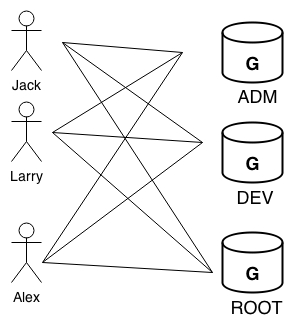
\includegraphics[width=0.3\textwidth]{assets/mediator_before}
	\caption{Objects communicating without using mediator pattern}
	\label{fig:mediator-before}
\end{figure}

\begin{figure}[H]
	\centering
	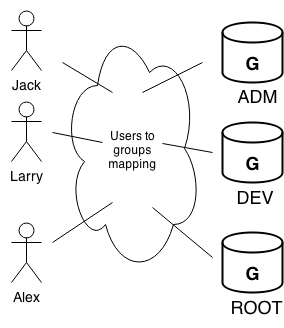
\includegraphics[width=0.3\textwidth]{assets/mediator_after}
	\caption{Objects communicating using mediator pattern}
	\label{fig:mediator-after}
\end{figure}

As seen in figure \ref{fig:mediator-before}, complexity of interactions between objects become exponentially large as the software grows.
\bs
Such problem occurs often in UI: An example would be when a input signal is mapped to multiple elements. In particular, say we have a button to open up the game menu. Then at the same time there are a few systems we need to talk to during this. First, we need to tell the game to lock all inputs to the character in the world, so that when we're navigating the menu, we don't move the character around. We want to enable mouse cursor (and hide it during game play). We might want to pause the game so that enemies don't attack in the background while we have the menu open. We might want to optimize performance by turning off rendering of the world when we're in the menu, since we might not able to see it anyway.
\bs
Without using a mediator, the activated event from the button would need to invoke methods in all these different systems. This \textit{antipattern} breaks abstraction, tightly decouples all these systems together which makes it prone to error and crashes, and makes the code highly unmaintainable.
\bs
Instead, we use pattern as depicted in figure \ref{fig:mediator-after}. The button event should communicate with a middle-man that sets a state. The various systems that would be affected does not know anything about the button, or anything that interacts with the mediator. It merely gets the state stored in the mediator, and performs corresponding action.
\bs

% CHANGED: this may not be the case as shared lock is more of a 'critical system' solution
% In Frostbite, a similar mechanism is called a \textit{SharedLock}. 

\subsection{Memento}

Memento are design patterns for objects to know how to save and load (externalize) its own internal state and data.\bs
\\
Usability improvement: when used together with Command pattern, we can create undo/redo actions. Not as applicable in the game engine itself, but essential to the development tools and editors artists and scripters use to develop the game.\bs
\\

\textbf{Difference Between Command and Memento}\bs
\\

Command passes a request from the client to be handled while memento passes its own internal state. Using an analogy of how a player interacts in a game menu: a command would be the event of player clicking on the save/load buttons of their game files, and the memento would be the save file objects itself being saved/loaded.\bs
\\

\subsection{Observer}

The observer design pattern is ubiquitous to software development. Observers define a one-to-many dependency where many clients can ``subscribe'' to a state change of a particular object. The clients would be notified by the broadcast sent by the subscribed object.\bs
\\
In observer pattern, the object sending the events is the \textit{subject}, and the objects receiving are the \textit{observer}. The observer hierarchy consists of an abstract \textit{observer} base class, which has some handler (see figure \ref{fig:observer-simple}).

\begin{figure}[H]
	\centering

	\scalebox{0.75}{
		\begin{tikzpicture}
			\begin{class}[text width=8cm]{Subject}{0,0}
				\attribute{-observers: ObserverBase[]}
				\operation{+Subject():}
				\operation{+RegisterObserver(ObserverBase *observer):}
				\operation{+UnregisterObserver(ObserverBase *observer):}
				\operation{-fireEvent(...):}
			\end{class}

			\begin{interface}{ObserverBase}{0,-5}
				\operation[0]{+handleEvent(...);}
			\end{interface}

			\begin{class}{ConcreteObserver}{0, -8}
				\implement{ObserverBase}
				\operation{+handleEvent(...):}
			\end{class}

			\draw[->](Subject)--node[right, black]{$<<$broadcasts$>>$}(ObserverBase);
		\end{tikzpicture}
	}

	\caption{Simple subject-object relationship in observer design pattern}
	\label{fig:observer-simple}
\end{figure}

Without using any mediators, the subject is \textit{loosely coupled}\footnote{Loose coupling means dependency to another object via interface or abstract class. Whereas tight coupling means dependency to the concrete class directly.} to the observer types. The subject holds a collection or list of registered observers, such that when an event should be fired, the subject iterates through all the observers and deliver the event.\bs
\\
The client is responsible for managing the observers' lifetime. The client or observers are responsible for when to register or unregister to a subject. In essence, the subject makes no assumption about its observers. (Similar to the relationship in model-view-controller where the controller act as observer to the view to enable user interaction - see section \ref{ssection:ecs}).\bs
\\
In Frostbite (and extends to many game engines and software), many OOP and inter-class relationship relies on events. A player's interaction with the controller, keyboard, or mouse triggers input events to be handled by the Input Handler. For example shown in figure \ref{fig:unreal-input}, the subject are objects that outputs an event whenever certain key is pressed (red blocks). The output event \textit{Released} is hooked up to some observer. The corresponding observers are the \textit{Move Updated Component} handlers that carries out specific tasks whenever it receives the event/signal.

\begin{figure}[H]
	\centering
	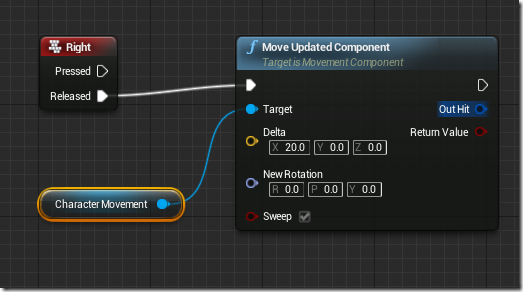
\includegraphics[width=0.49\textwidth]{assets/unreal-input}
	\caption{Example of event connections in Unreal Engine which is based on the observer design pattern. \cite{gfs-input}}
	\label{fig:unreal-input}
\end{figure}

It avoids the antipattern of \textit{spaghetti code} where increase in complexity of the software leads to exponential increase in complexity and unmaintainable code. The design pattern is very useful for organization, maintainability, flexibility, and scalability of code.\bs
\\
There are several approach to the implementation. Mainly, the subject could push data to observers during the function call. Or the observers could pull data from the subject. The observers could receive a subject pointer during construction and register themselves, or a client could register the observers for them. Nonetheless, the observer pattern is flexible and fit many needs in video game programming.\bs
\\
A sample code of an observer pattern example is in section \ref{code:observer}. In this example, we created a simple system to broadcast world events to a multiplayer game.

\subsection{Visitor}
TODO:


% Two columns end
\iftwocolumns
\end{multicols}
\fi